\documentclass[a4paper,12pt]{article}
\usepackage[utf8]{inputenc}
\usepackage[T1]{fontenc}
\usepackage[ngerman]{babel}
\usepackage{graphicx}
\usepackage{geometry}
\usepackage{hyperref}
\usepackage{enumitem}

\geometry{a4paper, margin=1in}

\title{Milestone 1: Infrastruktur-Spezifikation}
\author{Hammerschmidt, Rentenberger, Schodl, Weidinger}
\date{\today}

\begin{document}

\maketitle
\tableofcontents
\newpage

\section{Netzwerktopologie}

\begin{figure}[h!]
    \centering
    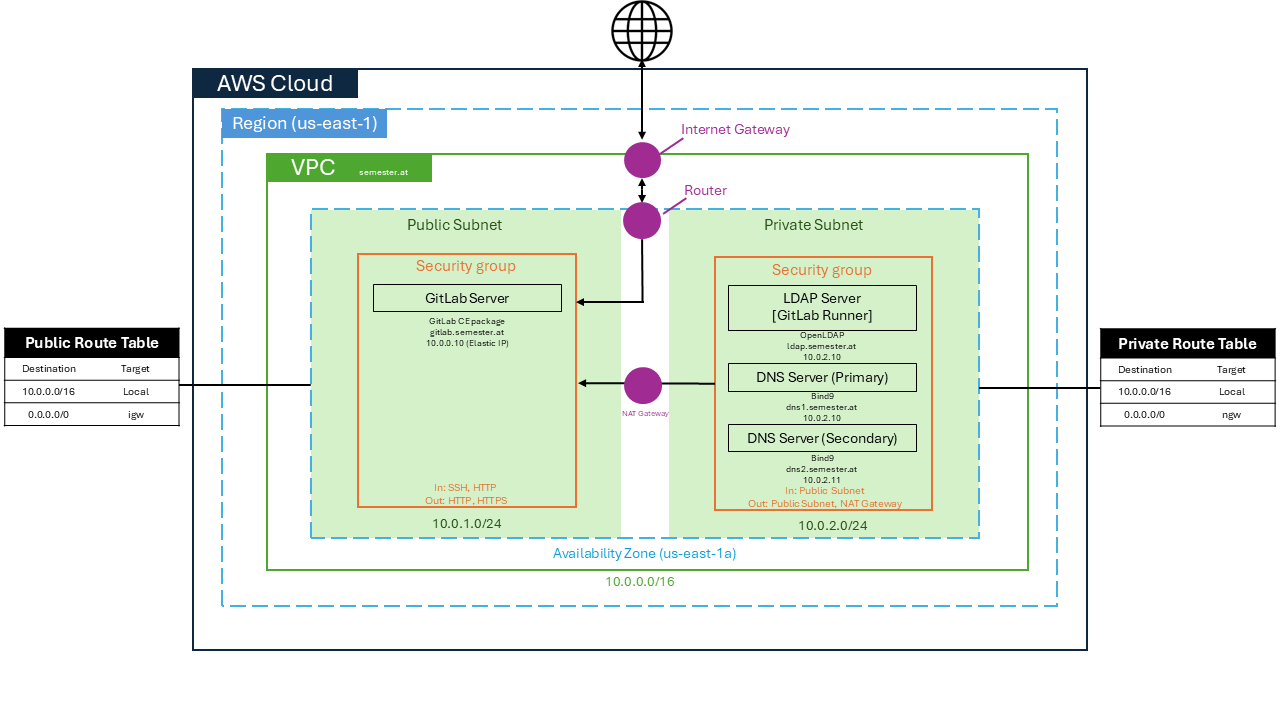
\includegraphics[width=\textwidth]{data/DevOps_Network_Topology.png}
    \caption{Netzwerktopologie der Infrastruktur}
    \label{fig:network_topology}
\end{figure}

\begin{table}[h!]
    \centering
    \begin{tabular}{|l|l|l|l|}
    \hline
    \textbf{Dienst}          & \textbf{Subnetztyp}      & \textbf{IP-Adresse} & \textbf{FQDN}             \\ \hline
    Primärer DNS             & Privates Subnetz         & 10.0.1.10                & dns1.semester.at         \\ \hline
    Sekundärer DNS           & Privates Subnetz         & 10.0.1.11                & dns2.semester.at         \\ \hline
    GitLab Server            & Öffentliches Subnetz     & 10.0.0.10                & gitlab.semester.at       \\ \hline
    LDAP Server              & Privates Subnetz         & 10.0.2.10                & server-ldap.semester.at         \\ \hline
    \end{tabular}
    \caption{Netzwerkdienste und IP-Zuordnung}
\end{table}

\section{Geplante Security Groups und Regeln}
Die Security Groups definieren, welche Dienste und Ports erreichbar sind:

\begin{table}[h!]
    \centering
    \begin{tabular}{|l|l|l|}
    \hline
    \textbf{Dienst}      & \textbf{Eingehend (Ingress)}          & \textbf{Ausgehend (Egress)}         \\ \hline
    DNS                 & Port 53 (UDP/TCP) von privatem Subnetz & Alle Ports ins VPC-Netz             \\ \hline
    GitLab              & Port 80/443 (HTTP/HTTPS) von bestimmten IPs & Alle Ports ins VPC-Netz             \\ \hline
    GitLab Runner       & Port 8093 von GitLab-Server            & Alle Ports ins VPC-Netz             \\ \hline
    LDAP                & Port 389 (LDAP) nur aus privatem Subnetz & Alle Ports ins VPC-Netz             \\ \hline
    \end{tabular}
    \caption{Geplante Security Groups und Regeln}
\end{table}

\begin{table}[h!]
    \centering
    \begin{tabular}{|l|c|c|c|c|}
    \hline
    \textbf{Inbound SGRs} & \textbf{DNS}              & \textbf{Bastion}         & \textbf{LDAP/GitLab-R}    & \textbf{GitLab-Server}    \\ \hline
    HTTP                  & Nein                      & Nein                     & Nein                      & Ja (0.0.0.0/0)           \\ \hline
    HTTPS                 & Nein                      & Nein                     & Ja (10.0.0.0/24)          & Ja (0.0.0.0/0)           \\ \hline
    SSH                   & Ja (10.0.0.0/24)          & Ja (0.0.0.0/0)           & Ja (0.0.0.0/0)            & Ja (0.0.0.0/0)           \\ \hline
    DNS (UDP)             & Ja (10.0.0.0/24)          & Nein                     & Nein                      & Nein                     \\ \hline
    DNS (TCP)             & Ja (10.0.0.0/24)          & Nein                     & Nein                      & Nein                     \\ \hline
    LDAP                  & Nein                      & Nein                     & Ja (0.0.0.0/0)            & Ja (0.0.0.0/0)           \\ \hline
    ALL ICMP              & Ja (0.0.0.0/0)            & Nein                     & Nein                      & Ja (10.0.0.0/24)         \\ \hline
    \end{tabular}
    \caption{Eingehende Sicherheitsgruppenregeln (SGRs) für verschiedene Dienste}
    \label{tab:inbound-sgrs}
\end{table}

\begin{table}[h!]
    \centering
    \begin{tabular}{|l|c|c|c|c|}
    \hline
    \textbf{Outbound SGRs} & \textbf{DNS}              & \textbf{Bastion}         & \textbf{LDAP/GitLab-R}    & \textbf{GitLab-Server}    \\ \hline
    HTTP                   & Nein                      & Nein                     & Ja (0.0.0.0/0)            & Nein                     \\ \hline
    HTTPS                  & Nein                      & Nein                     & Ja (0.0.0.0/0)            & Nein                     \\ \hline
    SSH                    & Nein                      & Nein                     & Ja (0.0.0.0/0)            & Nein                     \\ \hline
    DNS (UDP)              & Nein                      & Nein                     & Ja (0.0.0.0/0)            & Nein                     \\ \hline
    DNS (TCP)              & Nein                      & Nein                     & Ja (0.0.0.0/0)            & Nein                     \\ \hline
    LDAP                   & Nein                      & Nein                     & Ja (0.0.0.0/0)            & Ja (0.0.0.0/0)           \\ \hline
    ALL ICMP               & Nein                      & Nein                     & Ja (0.0.0.0/0)            & Nein                     \\ \hline
    ALL Traffic            & Ja (0.0.0.0/0)            & Ja (0.0.0.0/0)           & Nein                      & Ja (0.0.0.0/0)           \\ \hline
    \end{tabular}
    \caption{Ausgehende Sicherheitsgruppenregeln (SGRs) für verschiedene Dienste}
    \label{tab:outbound-sgrs}
\end{table}

\section{Dienste-Zuordnung zu Server-Instanzen}

\begin{table}[h!]
    \centering
    \begin{tabular}{|l|l|l|}
    \hline
    \textbf{Serverinstanz} & \textbf{Betriebssystem}  & \textbf{Dienste}         \\ \hline
    DNS-Server 1           & Ubuntu 22.04 LTS        & BIND (Primärer DNS)      \\ \hline
    DNS-Server 2           & Ubuntu 22.04 LTS        & BIND (Sekundärer DNS)    \\ \hline
    GitLab Server          & Ubuntu 22.04 LTS        & GitLab CE                \\ \hline
    GitLab Runner          & Ubuntu 22.04 LTS        & GitLab Runner            \\ \hline
    LDAP Server            & Ubuntu 22.04 LTS        & OpenLDAP                 \\ \hline
    \end{tabular}
    \caption{Dienste-Zuordnung zu Server-Instanzen}
\end{table}

\section{Spezifikationen der eingesetzten Systeme}

\begin{table}[h!]
    \centering
    \begin{tabular}{|l|l|l|l|l|}
    \hline
    \textbf{Server}               & \textbf{OS}                 & \textbf{Packages}          & \textbf{Version}                     & \textbf{Server Instance} \\ \hline
    Preferred DNS Server          & Ubuntu Server              & bind9, bind9utils          & BIND 9.18.19 / Ubuntu 22.04.3 LTS    & T3.micro                \\ \hline
    Alternative DNS Server        & Ubuntu Server              & bind9, bind9utils          & BIND 9.18.19 / Ubuntu 22.04.3 LTS    & T3.micro                \\ \hline
    LDAP Server                   & Ubuntu Server              & slapd, ldap-utils          & OpenLDAP 2.6.6                       & T3.micro                \\ \hline
    GitLab Runner                 & Ubuntu Server              & -                          & Ubuntu 22.04.3 LTS                   & T3.micro                \\ \hline
    GitLab Server                 & Ubuntu Server              & GitLab CE                  & GitLab CE / Ubuntu 22.04.3 LTS       & T2.Large                \\ \hline
    \end{tabular}
    \caption{Server-Spezifikationen: Betriebssystem, Pakete und Instanztypen}
    \label{tab:server-specs}
\end{table}
    
\begin{itemize}
    \item \textbf{Betriebssystem}: Ubuntu 22.04 LTS (64-bit)
    \item \textbf{DNS-Server}: BIND 9.18
    \item \textbf{GitLab}: GitLab CE 15.x
    \item \textbf{GitLab Runner}: Version kompatibel mit GitLab CE 15.x
    \item \textbf{LDAP}: OpenLDAP 2.5.x
    \item \textbf{Optionale Überwachung}: AWS CloudWatch zur Protokollierung und Überwachung.
\end{itemize}

\section{Tests}
\subsection*{DNS Resolution Testing}
\begin{itemize}[leftmargin=1.5cm]
    \item \textbf{Objective:} Ensure the BIND server correctly resolves domain names.
    \item \textbf{Method:} Use the \texttt{dig} command to query the DNS server for known domains. Check \texttt{A}, \texttt{AAAA}, \texttt{MX}, and \texttt{NS} records:
    \begin{verbatim}
    dig @<DNS-server> example.com [A, AAAA, MX, NS]
    \end{verbatim}
    \item \textbf{Expected Outcome:} Each query returns the correct IP addresses and record details.
\end{itemize}

\subsection*{Forward and Reverse DNS Lookup}
\begin{itemize}[leftmargin=1.5cm]
    \item \textbf{Objective:} Verify that forward and reverse lookups are functional.
    \item \textbf{Method:}
    \begin{itemize}
        \item Use \texttt{dig} for forward lookup (domain to IP):
        \begin{verbatim}
        dig @<DNS-server> example.com A
        \end{verbatim}
        \item Use \texttt{dig -x} for reverse lookup (IP to domain):
        \begin{verbatim}
        dig @<DNS-server> -x [192.0.2.1]
        \end{verbatim}
    \end{itemize}
    \item \textbf{Expected Outcome:} Accurate mapping between domain names and IP addresses.
\end{itemize}

\subsection*{Zone Transfer Test}
\begin{itemize}[leftmargin=1.5cm]
    \item \textbf{Objective:} Ensure zone transfers between primary and secondary DNS servers are working.
    \item \textbf{Method:} Initiate a zone transfer using \texttt{dig AXFR} and check logs for the transfer:
    \begin{verbatim}
    dig @<primary-DNS-server> example.com AXFR
    \end{verbatim}
    \item \textbf{Expected Outcome:} Zone data is accurately replicated between primary and secondary servers.
\end{itemize}

\subsection*{DNS Failover Testing}
\begin{itemize}[leftmargin=1.5cm]
    \item \textbf{Objective:} Assess the resilience and reliability of the DNS service under failure conditions.
    \item \textbf{Method:}
    \begin{itemize}
        \item Simulate a failure of the primary DNS server.
        \item Monitor the response from the secondary DNS server:
        \begin{verbatim}
        dig @<secondary-DNS-server> example.com A
        \end{verbatim}
        \item Record any downtime experienced during the transition.
    \end{itemize}
    \item \textbf{Expected Outcome:} The secondary DNS server seamlessly takes over with little to no disruption in DNS resolution.
\end{itemize}

\subsection*{Stress Testing}
\begin{itemize}[leftmargin=1.5cm]
    \item \textbf{Objective:} Test the performance of the server under high load.
    \item \textbf{Method:} Use tools such as \texttt{dnsperf} to simulate a high number of DNS queries:
    \begin{verbatim}
    dnsperf -s <primary-DNS-IP> -d queries.txt -l 30
    \end{verbatim}
    \item \textbf{Expected Outcome:} The server maintains accuracy and performs well under the load.
\end{itemize}

\section{Rollen und Verantwortlichkeiten im Team}
\begin{table}[h!]
    \centering
    \begin{tabular}{|l|l|}
    \hline
    \textbf{Rolle}            & \textbf{Verantwortlichkeiten}               \\ \hline
    Netzwerk-Architekt        & Planung und Einrichtung der VPC und Subnetze \\ \hline
    DevOps-Ingenieur          & Bereitstellung von GitLab und CI/CD         \\ \hline
    Systemadministrator       & Konfiguration von DNS- und LDAP-Servern     \\ \hline
    QA-Ingenieur              & Testen der Dienste und Sicherheitskonfiguration \\ \hline
    \end{tabular}
    \caption{Rollen und Verantwortlichkeiten}
\end{table}

\section{FQDN und interne Domain}
Die interne Domain wird als \textbf{intern.local} festgelegt. Beispiele:
\begin{itemize}
    \item DNS-Server: \texttt{dns1.intern.local}, \texttt{dns2.intern.local}.
    \item GitLab: \texttt{gitlab.intern.local}.
\end{itemize}

\section*{Optional: Monitoring}
AWS CloudWatch wird zur Protokollierung und Überwachung genutzt:
\begin{itemize}
    \item Überwachung der CPU-, Speicher- und Netzwerknutzung.
    \item Automatische Alarme bei Ausfällen.
\end{itemize}

\end{document}
